\documentclass[xcolor=dvipsnames]{beamer}
\usepackage[T1]{fontenc}
\usepackage[utf8]{inputenc}
\usepackage[english,slovak]{babel}

\usepackage{amsmath}
\usepackage{amsthm}
\usetheme{Pittsburgh}
\useoutertheme{shadow}

\usepackage{graphicx}
\usepackage{caption}
\usepackage{subcaption}

\usepackage[]{algorithm2e}
\usepackage{listings}
 \setbeamercovered{transparent}
 \usepackage{cuted}
\usepackage[export]{adjustbox}
\usepackage{mathtools}

\usepackage{lipsum}
\usepackage{verbatim}
\usepackage{transparent}
\usepackage{framed}
\usepackage{xcolor}

\usepackage{multirow}
\usepackage{colortbl}
\usepackage{lmodern}

\newcommand\Wider[2][3em]{%
\makebox[\linewidth][c]{%
  \begin{minipage}{\dimexpr\textwidth+#1\relax}
  \raggedright#2
  \end{minipage}%
  }%
}




\iftrue

\usetheme{Warsaw}

\setbeamercolor{normal text}{fg=white,bg=black!90}
\setbeamercolor{structure}{fg=white}

\setbeamercolor{alerted text}{fg=red!85!black}

\setbeamercolor{item projected}{use=item,fg=black,bg=item.fg!35}

\setbeamercolor*{palette primary}{use=structure,fg=structure.fg}
\setbeamercolor*{palette secondary}{use=structure,fg=structure.fg!95!black}
\setbeamercolor*{palette tertiary}{use=structure,fg=structure.fg!90!black}
\setbeamercolor*{palette quaternary}{use=structure,fg=structure.fg!95!black,bg=black!80}

\setbeamercolor*{framesubtitle}{fg=white}

\setbeamercolor*{block title}{parent=structure,bg=black!60}
\setbeamercolor*{block body}{fg=black,bg=black!10}
\setbeamercolor*{block title alerted}{parent=alerted text,bg=black!15}
\setbeamercolor*{block title example}{parent=example text,bg=black!15}

\fi



%-------------------------------------------------------------------------------------
\title{\color{white} \bf motoko uprising}
\author{\color{white} Michal CHOVANEC, PhD}


%\setbeamertemplate{footline}[frame number]{}
\setbeamertemplate{navigation symbols}{}


\date[EURP]{}
\begin{document}

{
    \usebackgroundtemplate
    {
        \vbox to \paperheight{\vfil\hbox to \paperwidth{\hfil

        {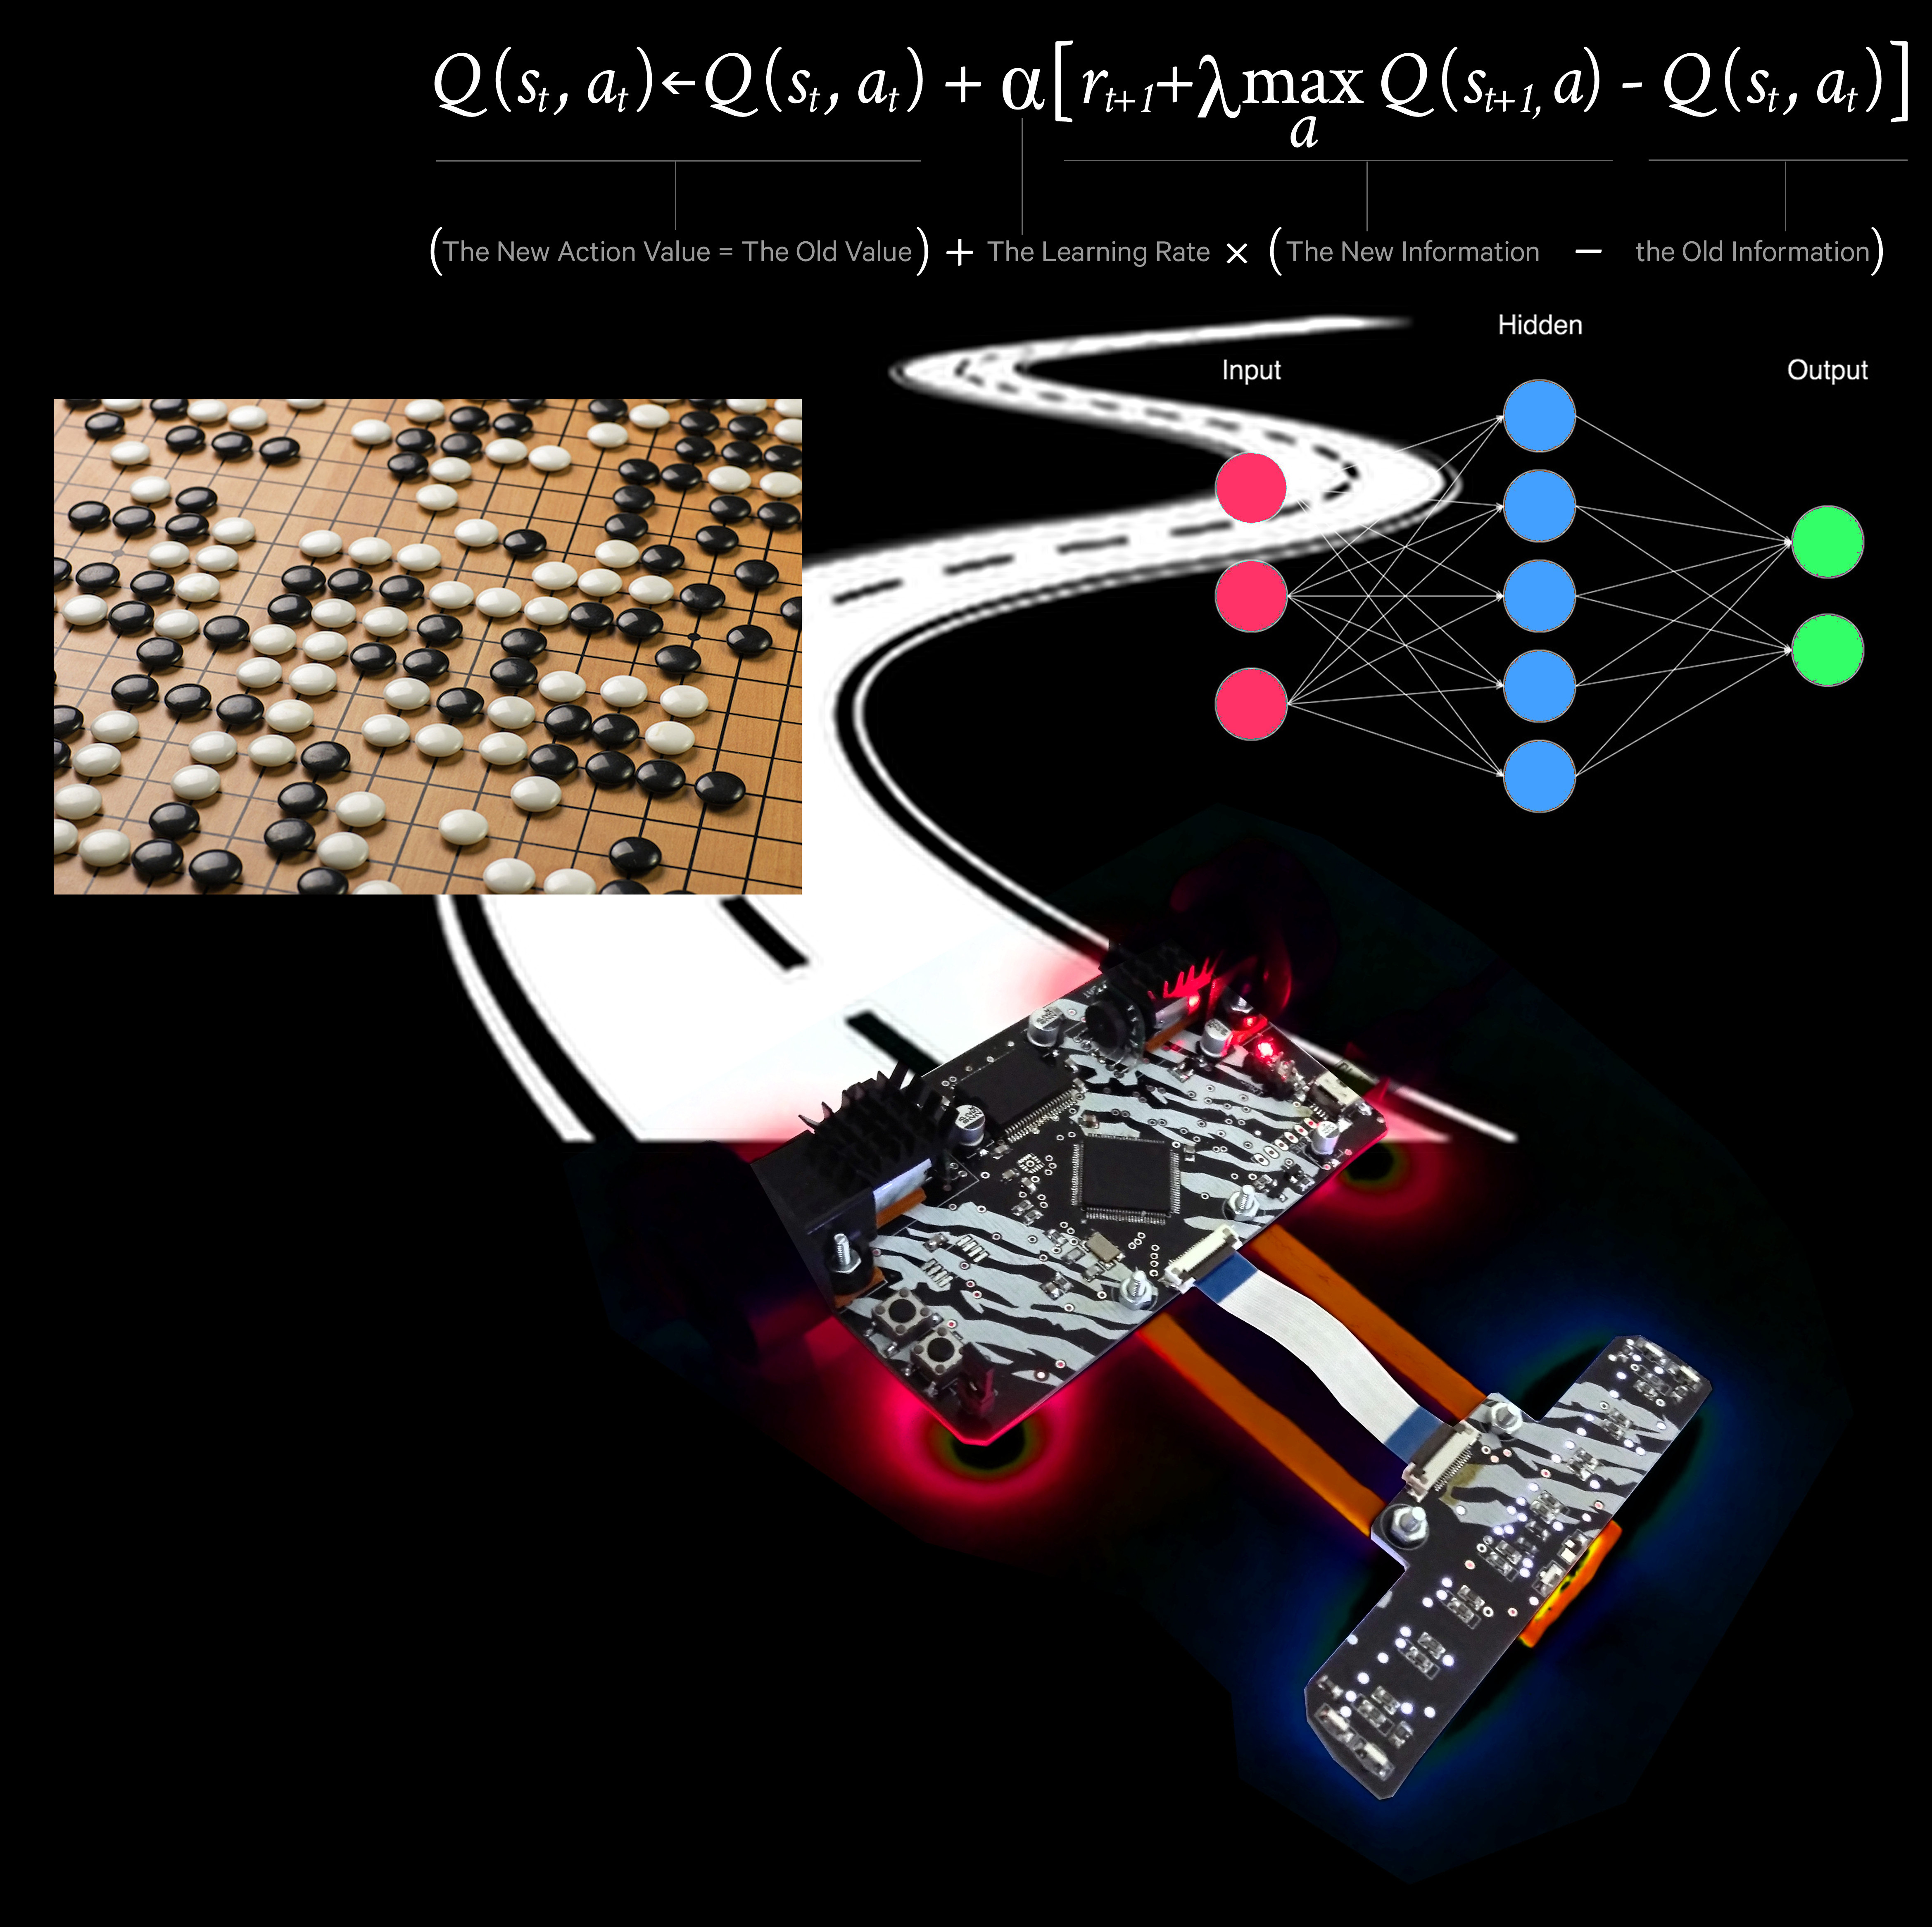
\includegraphics[width=5.05in]{../../pictures/rl_square.jpg}}

        \hfil}\vfil}
    }
    \begin{frame}

    %\titlepage


    \centering
     \colorbox{black}
     {
        \begin{minipage}{7cm}
           {\LARGE \color{white} {\bf MOTOKO UPRISING} \\ The line following robot} \\
           {\LARGE \color{white} Michal CHOVANEC, PhD} \\
       \end{minipage}
     }


    \end{frame}
}

\begin{frame}{\bf Line follower competition}


\begin{figure}
    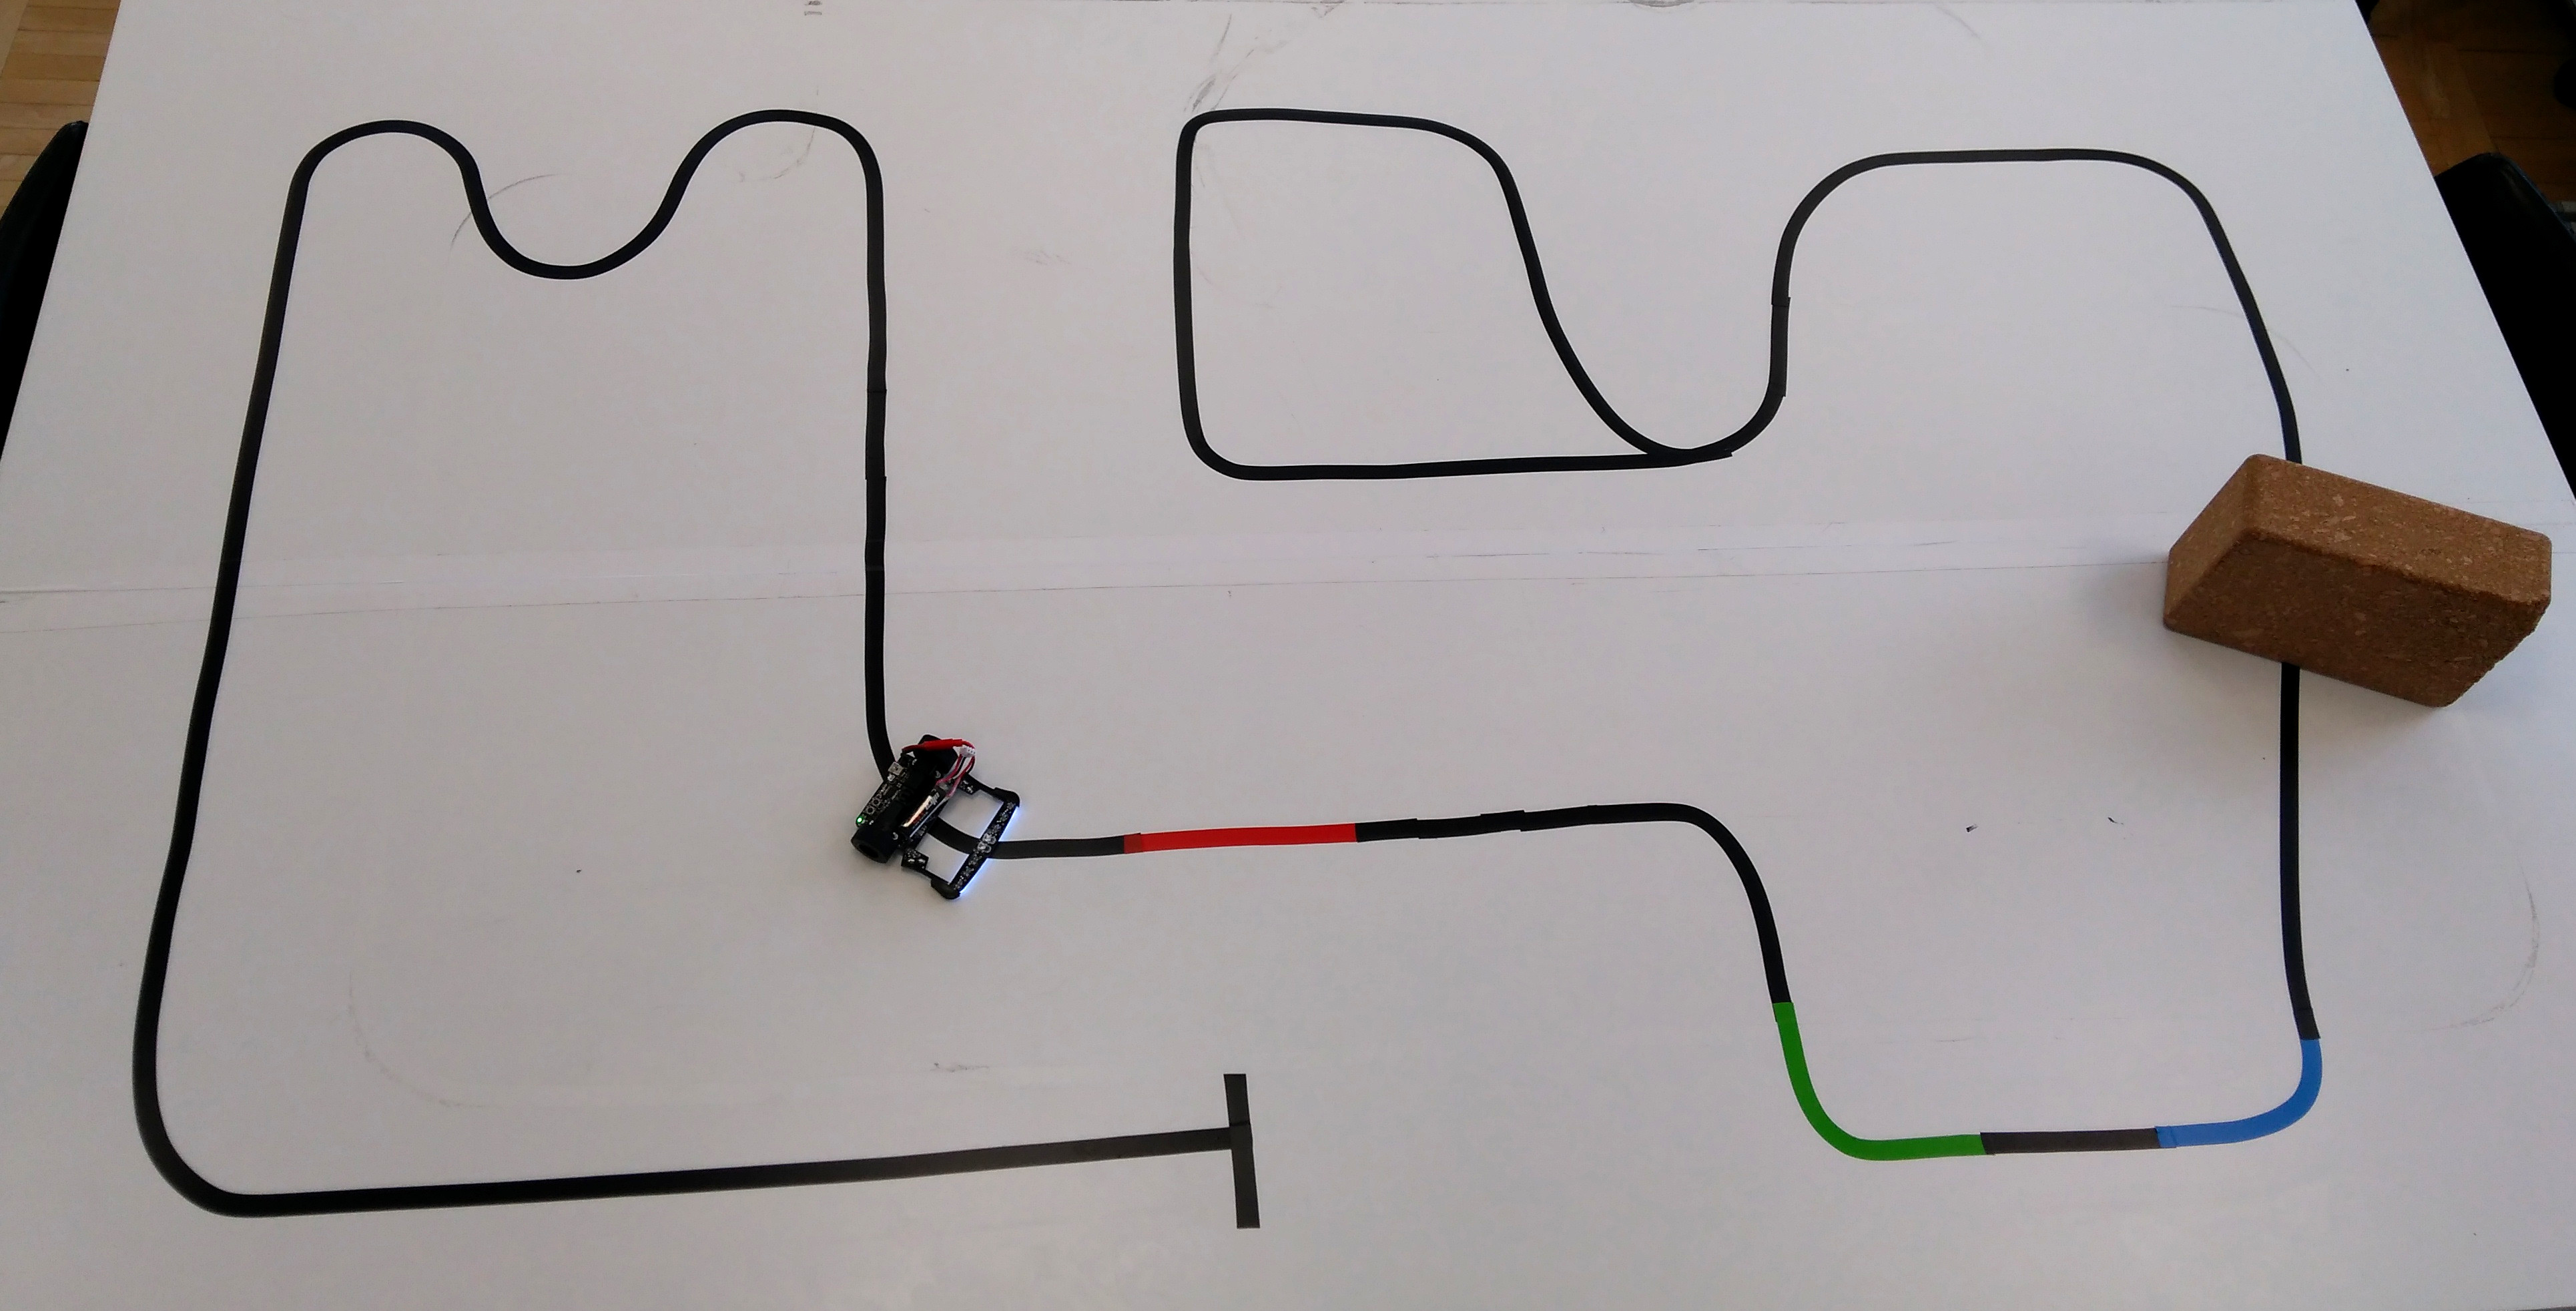
\includegraphics[scale=0.07]{../../pictures/motoko_uprising/line_follower.jpg}
\end{figure}

\begin{itemize}
    \item SR - Istrobot
    \item CR - Roboticky den
    \item AU - Robot Challenge
    \item PL - Zawody robotow
\end{itemize}


\end{frame}


\begin{frame}{\bf What does it take}

\begin{columns}

    \begin{column}{0.5\textwidth}

        \begin{itemize}
            \item Hardware
                \begin{itemize}
                    \item strong light motors
                    \item high adhesion tyres
                    \item light accumulator
                    \item fast CPU
                    \item dozen of sensors
                \end{itemize}
            \item Software
                \begin{itemize}
                    \item hard real time OS
                    \item tunned PIDs
                    \item predictive controll
                    \item mapping
                \end{itemize}
        \end{itemize}

    \end{column}

    \begin{column}{0.5\textwidth}

        \begin{figure}
            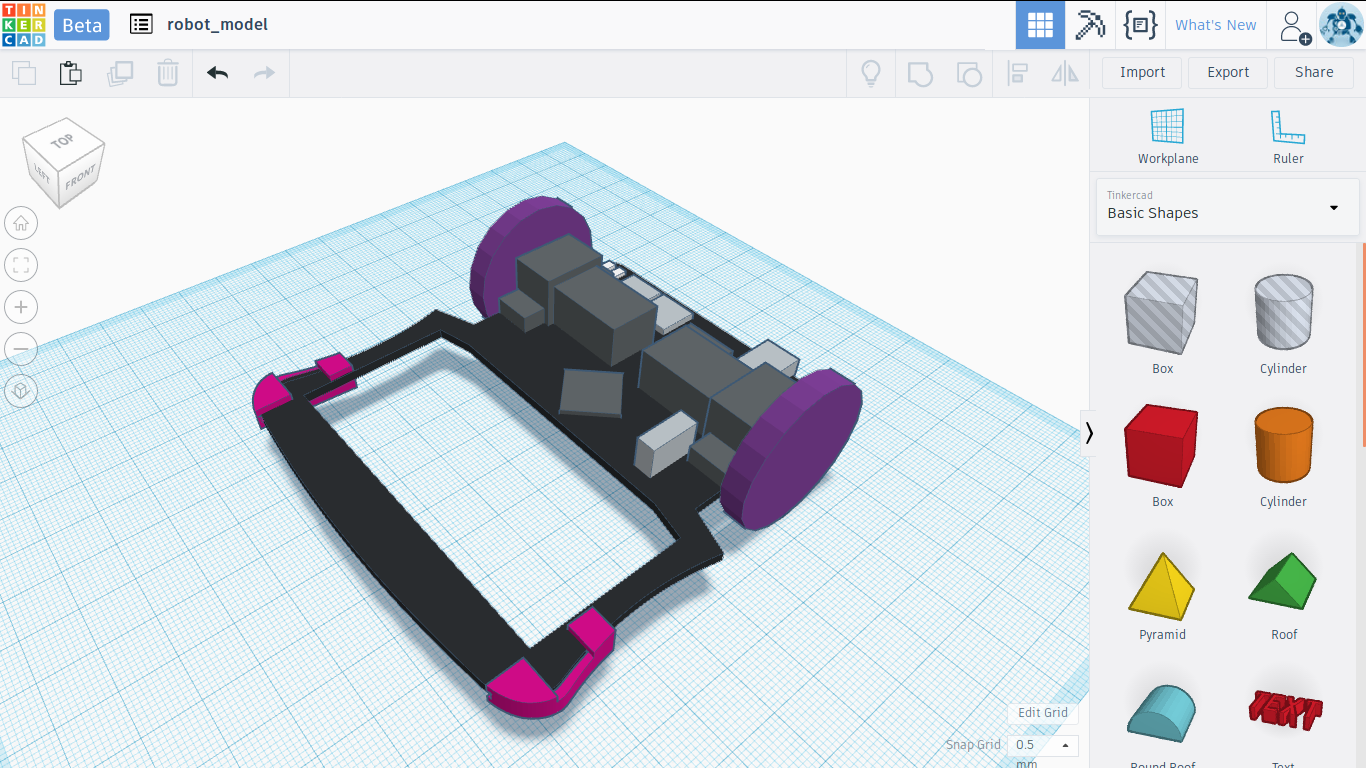
\includegraphics[scale=0.1]{../../pictures/motoko_uprising/robot_05.png}
        \end{figure}

        \begin{figure}
            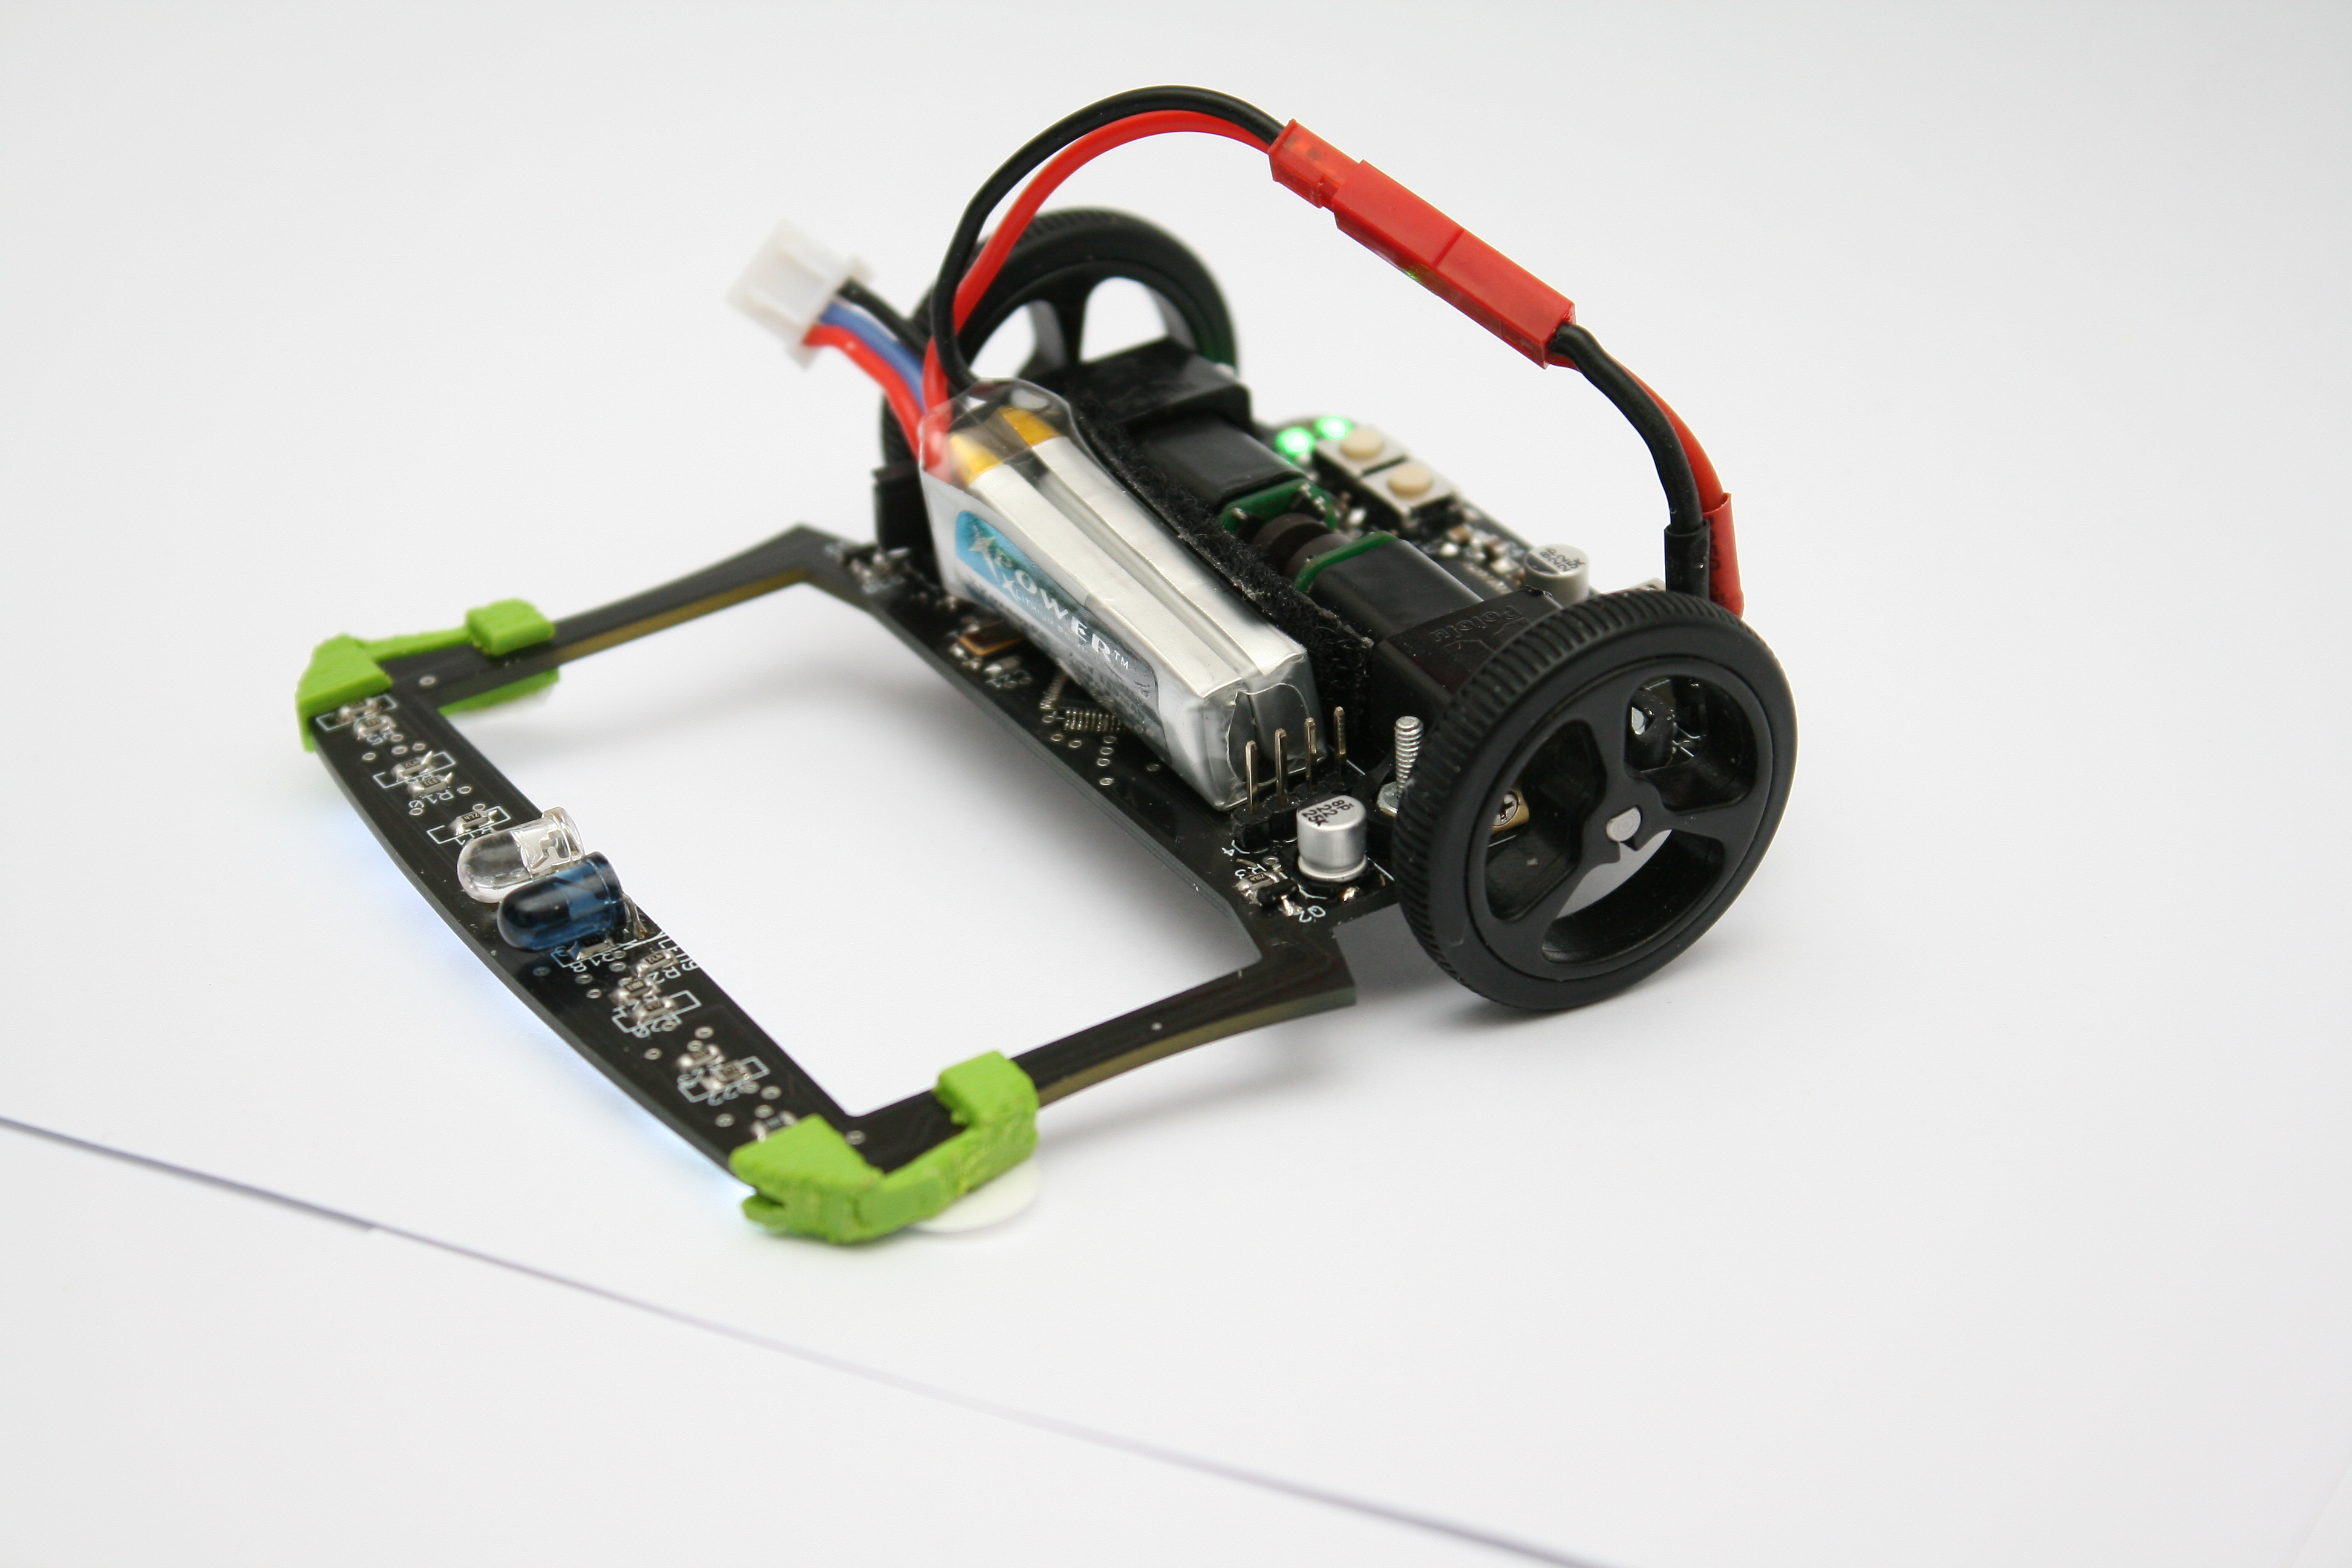
\includegraphics[scale=0.04]{../../pictures/motoko_uprising/robot_06.jpg}
        \end{figure}

    \end{column}


\end{columns}


\end{frame}


\begin{frame}{\bf Motoko uprising - hardware}


\begin{columns}

    \begin{column}{0.5\textwidth}

        \begin{figure}
            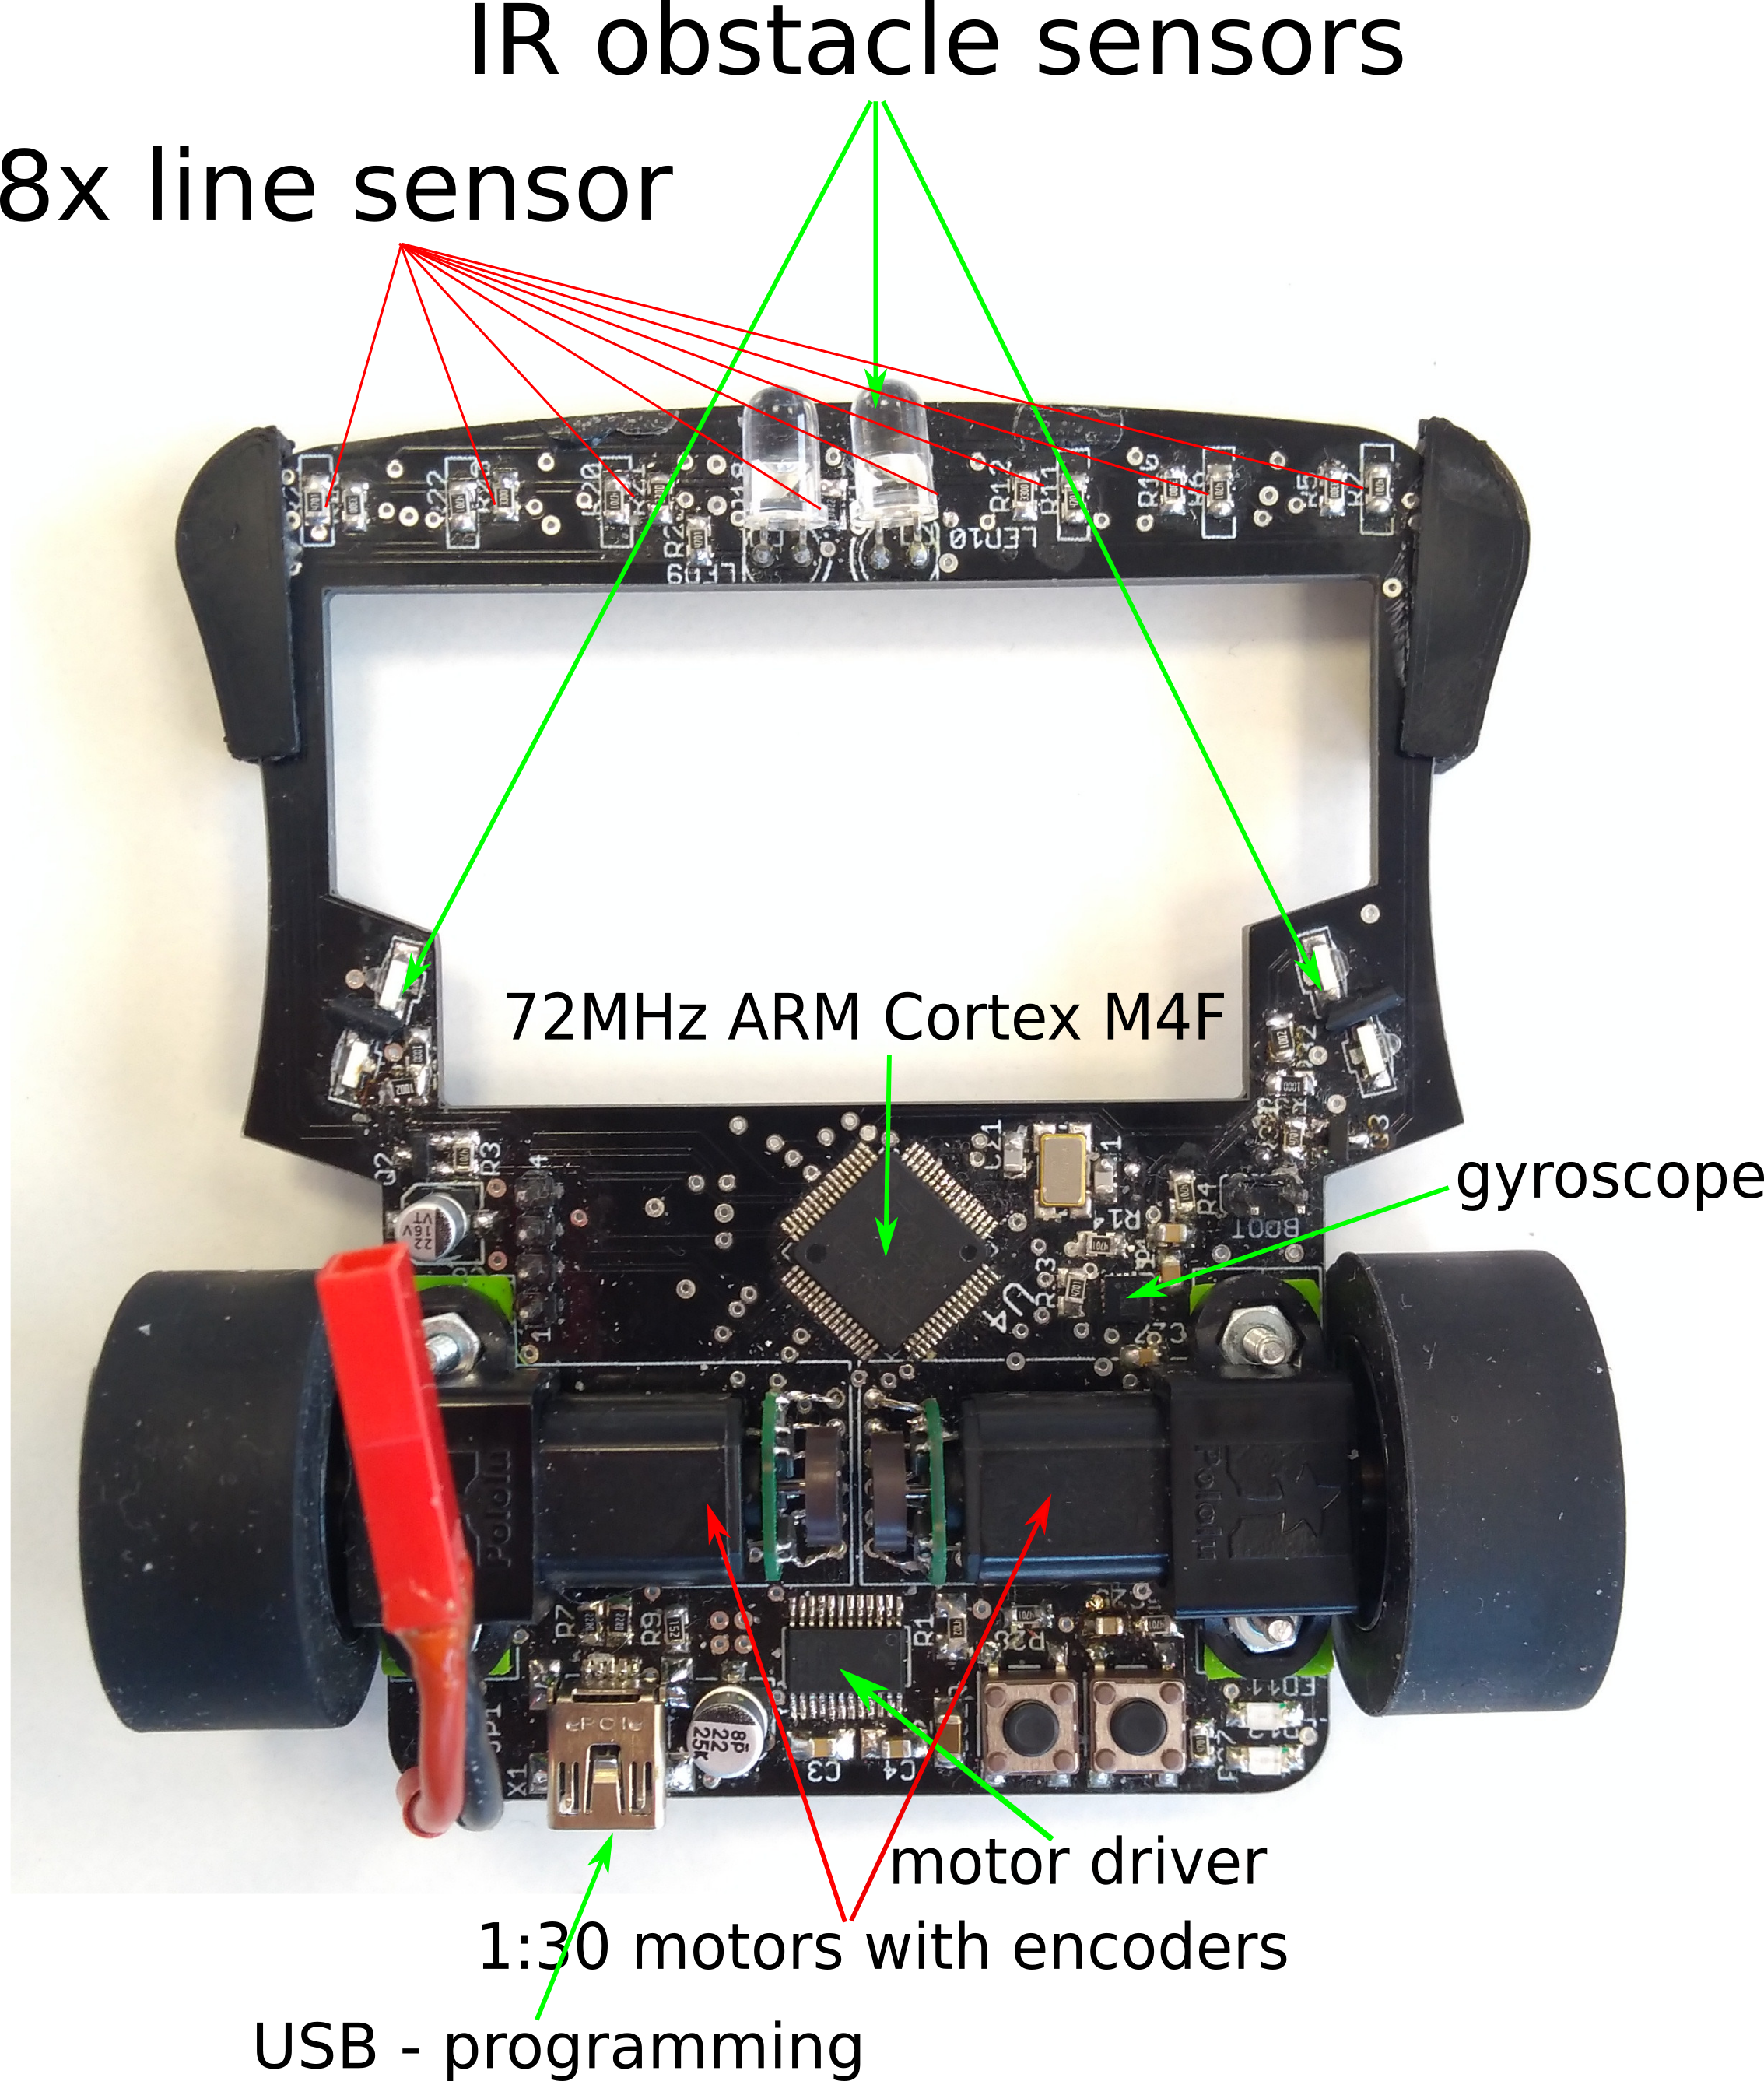
\includegraphics[scale=0.3]{../../diagrams/motoko_uprising_hw.png}
        \end{figure}

    \end{column}


    \begin{column}{0.5\textwidth}  %%<--- here
    {\small
        \begin{itemize}
            \item {\bf mcu}  : STM32F303, 72MHz ARM Cortex M4F
            \item {\bf motor driver} : TI DRV8834
            \item {\bf motors} : 1:30 HP Pololu, with magnetic encoder
            \item {\bf tyres} : Pololu 28mm diameter
            \item {\bf line sensor} : 8x 540nm phototransistor + white LED
            \item {\bf obstacle sensor} : SMD IR phototransistor + IR LED
            \item {\bf imu} : LSM6DS0, gyroscope + accelerometer
        \end{itemize}
    }
    \end{column}

\end{columns}


\end{frame}


\begin{frame}{\bf Software}



\begin{columns}

    \begin{column}{0.5\textwidth}  %%<--- here
    {\small
        \begin{itemize}
            \item {\bf quadratic interpolation}  : high precission line position computing
            \item {\bf steering PID}  : PD controller for steering
            \item {\bf motor PID}  : two PIDs for motors speed controll
            \item {\bf curve shape prediction}
                \begin{itemize}
                    \item {\bf fast} run on straight line, {\bf brake} on curve
                    \item {\color{red} \bf deep neural network}
                \end{itemize}
            \item written in {\bf C++}
            \item {\bf network training} on GPU - own framework for CNN
        \end{itemize}
    }
    \end{column}

    \begin{column}{0.5\textwidth}

        \begin{figure}
            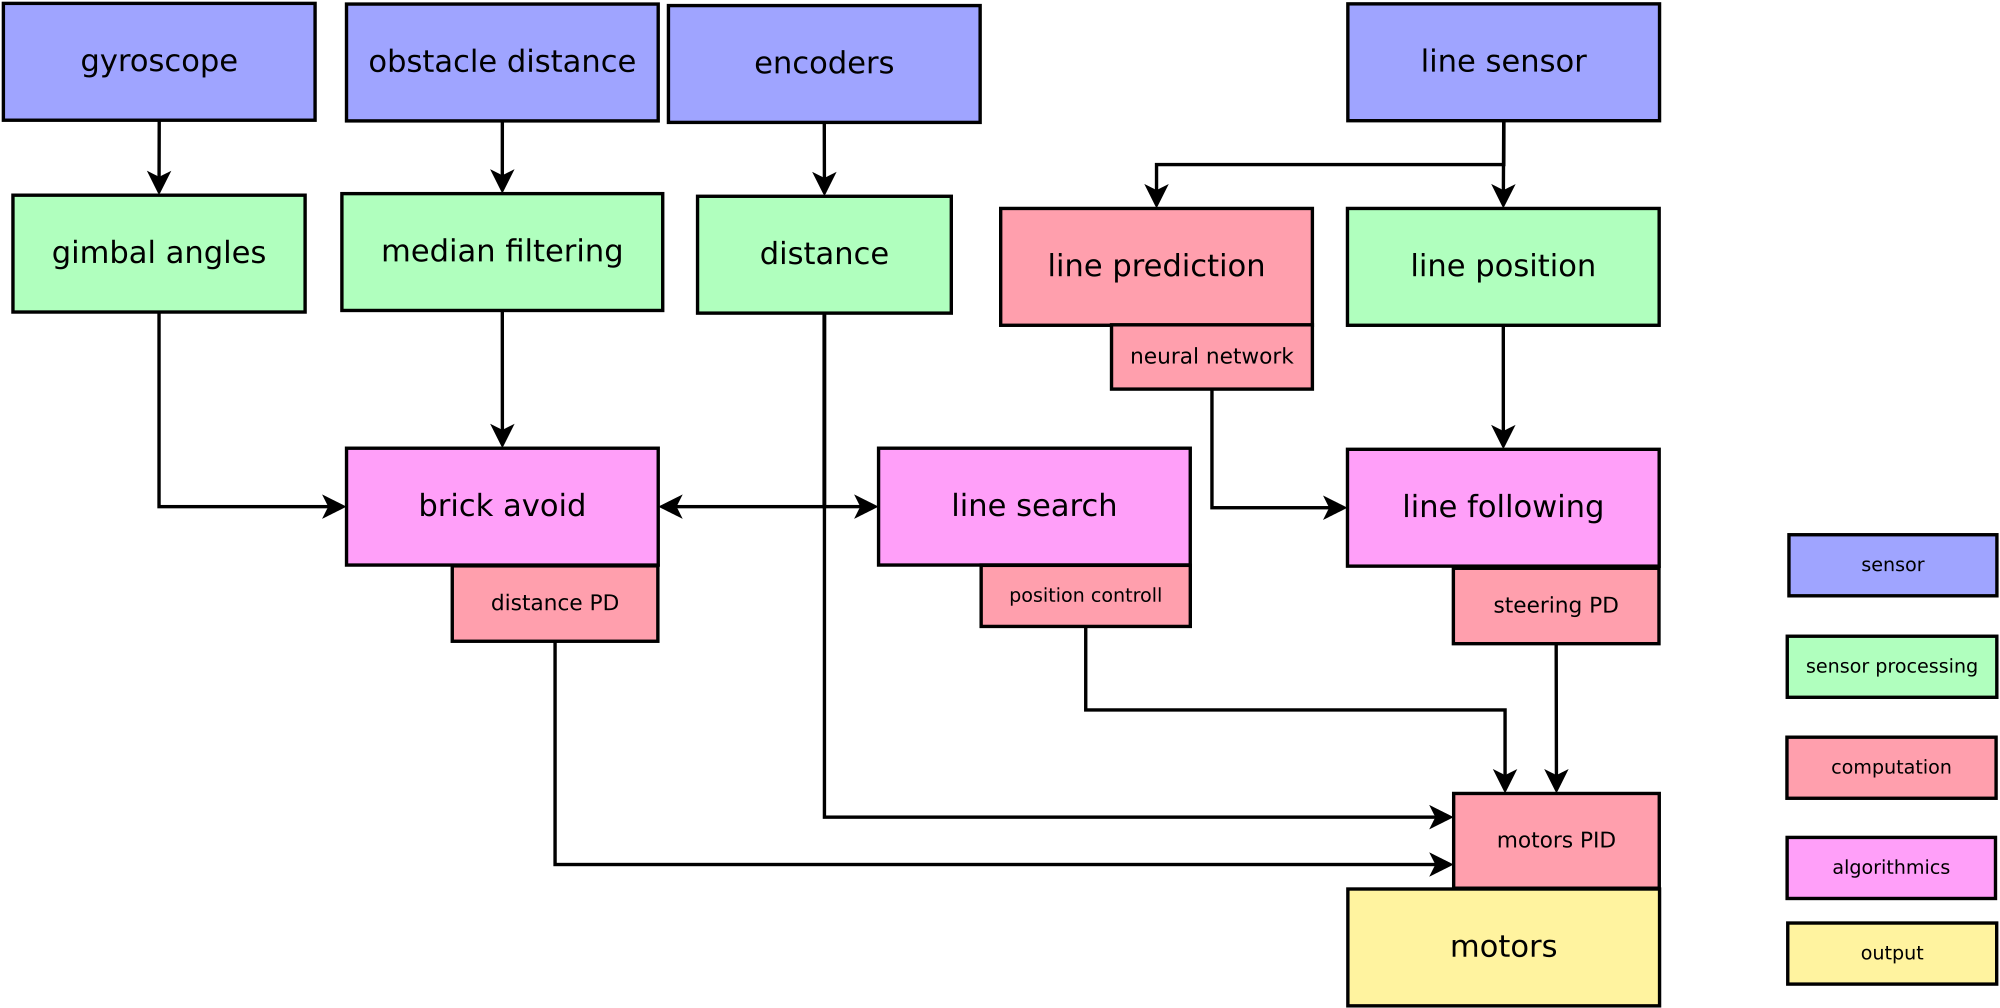
\includegraphics[scale=0.1]{../../diagrams/motoko_suftware_blocks.png}
        \end{figure}

    \end{column}




\end{columns}

\end{frame}


\begin{frame}{\bf Software}

\begin{figure}
    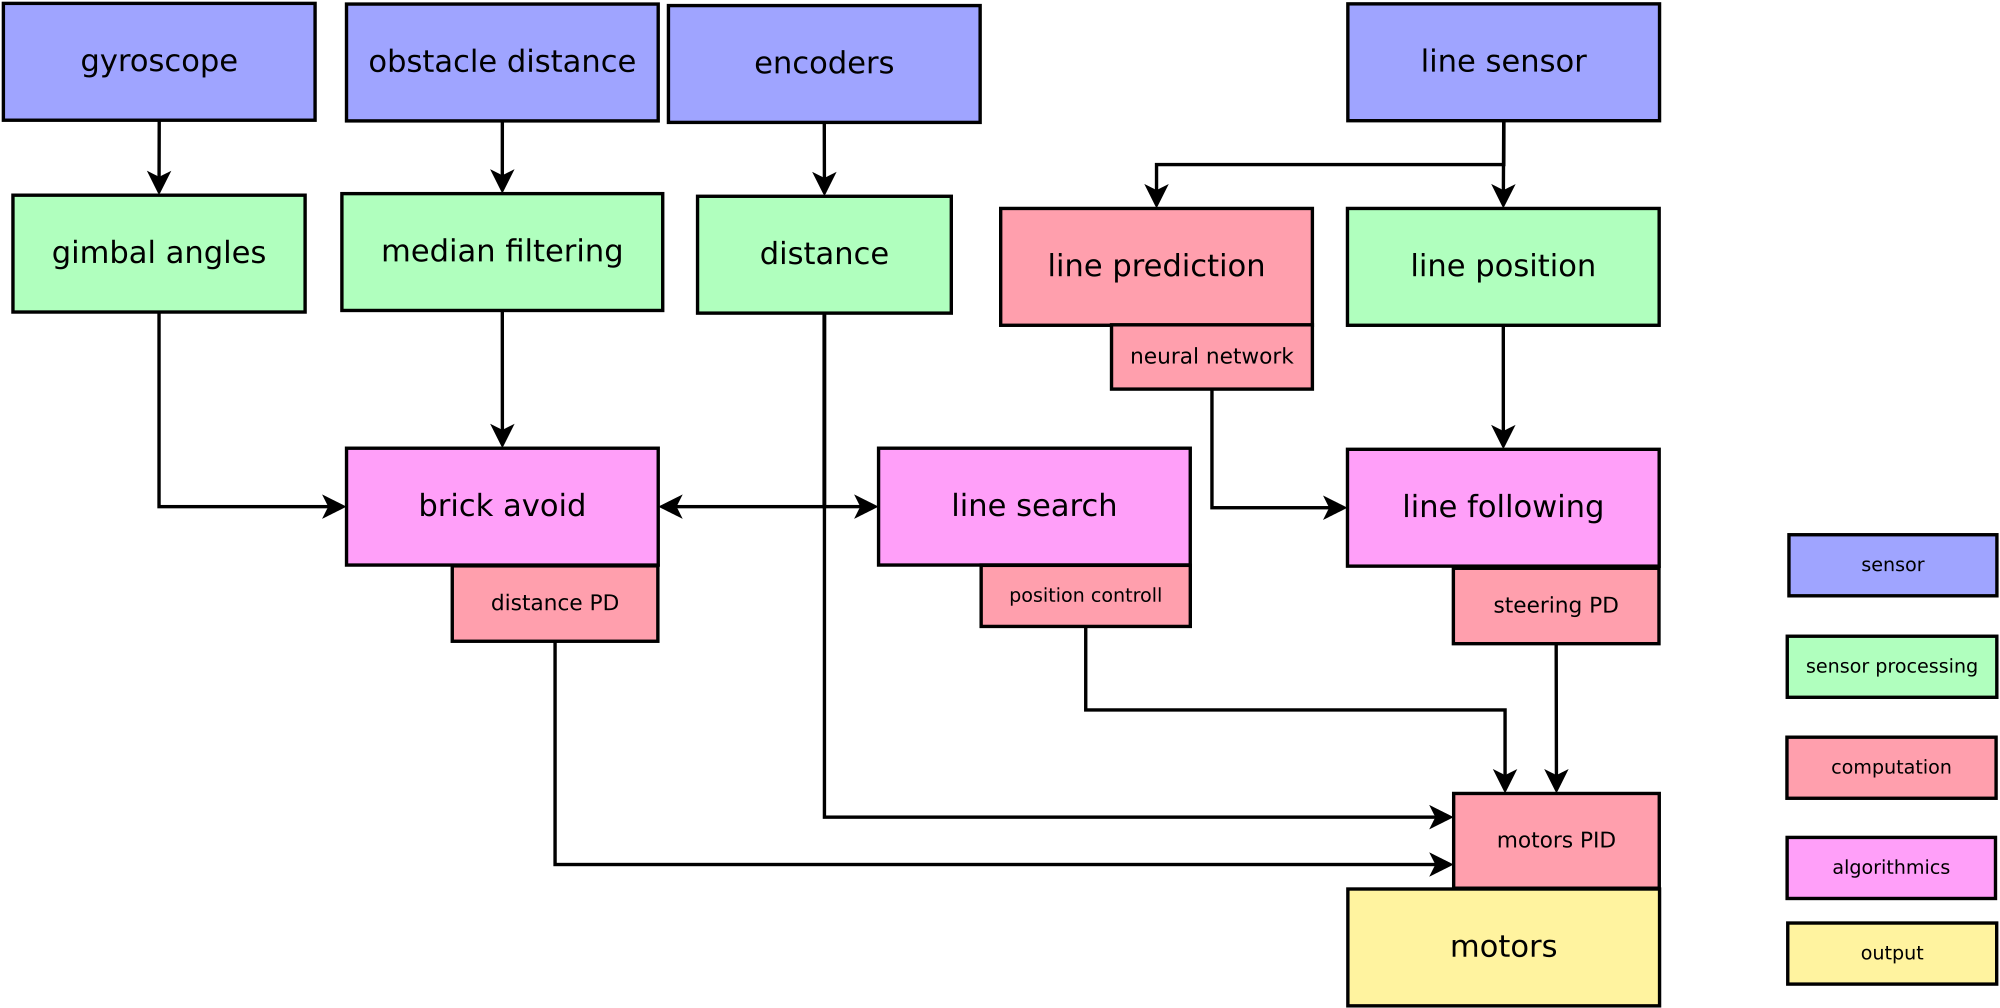
\includegraphics[scale=0.2]{../../diagrams/motoko_suftware_blocks.png}
\end{figure}


\end{frame}

\begin{frame}{\bf Line shape prediction}

\begin{itemize}
    \item {\bf fast} run on straight line, {\bf brake} on curve
    \item {\bf neural network} for line type classification
        \begin{itemize}
            \item DenseNet - densely connected convolutional neural network
        \end{itemize}
    \item {\bf input} 8x8 matrix raw data from line sensors
        \begin{itemize}
            \item 8 past line positions from 8 sensors
        \end{itemize}
    \item {\bf output} 5 curves types
\end{itemize}

\begin{figure}
    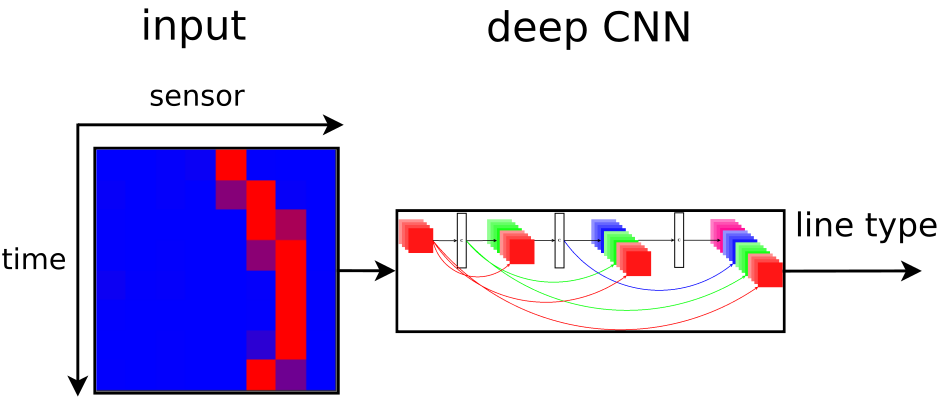
\includegraphics[scale=0.3]{../../diagrams/line_classification.png}
\end{figure}

\end{frame}


\begin{frame}{\bf Line dataset}


\begin{columns}

\begin{column}{0.5\textwidth}

    \begin{figure}
        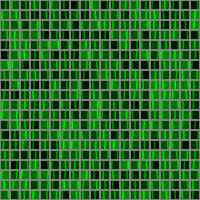
\includegraphics[scale=0.9]{../../pictures/line_follower_dataset.png}
    \end{figure}

\end{column}



\begin{column}{0.5\textwidth}  %%<--- here
{\small
    \begin{itemize}
        \item 20000 for training
        \item 2500 for testing
        \item 8x8 inputs
        \item 5 outputs (5 curves types)
            \begin{itemize}
                \item two left
                \item one straight
                \item two right
            \end{itemize}
        \item augmentation - luma noise, white noise

    \end{itemize}
}
\end{column}

\end{columns}



\end{frame}


\begin{frame}{\bf Neural networks architecture}

{\footnotesize

    \begin{table}[]
    \begin{tabular}{|c|l|l|l|l|}
    \hline
    \textbf{layer} & \multicolumn{1}{c|}{\textbf{net 0}}                                                 & \multicolumn{1}{c|}{\textbf{net 1}}                                                 & \multicolumn{1}{c|}{\textbf{net 2}}                                                 & \multicolumn{1}{c|}{\textbf{net 3}}                                                 \\ \hline
    \textbf{0}     & \cellcolor[HTML]{38FFF8}\begin{tabular}[c]{@{}l@{}}conv \\ 3x3x4\end{tabular}       & \cellcolor[HTML]{38FFF8}\begin{tabular}[c]{@{}l@{}}conv \\ 3x3x6\end{tabular}       & \cellcolor[HTML]{38FFF8}\begin{tabular}[c]{@{}l@{}}conv \\ 3x3x4\end{tabular}       & \cellcolor[HTML]{38FFF8}\begin{tabular}[c]{@{}l@{}}conv \\ 3x3x6\end{tabular}       \\ \hline
    \textbf{1}     & \cellcolor[HTML]{C0C0C0}\begin{tabular}[c]{@{}l@{}}max pooling \\ 2x2\end{tabular}  & \cellcolor[HTML]{C0C0C0}\begin{tabular}[c]{@{}l@{}}max pooling \\ 2x2\end{tabular}  & \cellcolor[HTML]{C0C0C0}\begin{tabular}[c]{@{}l@{}}max pooling \\ 2x2\end{tabular}  & \cellcolor[HTML]{C0C0C0}\begin{tabular}[c]{@{}l@{}}max pooling \\ 2x2\end{tabular}  \\ \hline
    \textbf{2}     & \cellcolor[HTML]{FD6864}\begin{tabular}[c]{@{}l@{}}dense conv \\ 3x3x4\end{tabular} & \cellcolor[HTML]{FD6864}\begin{tabular}[c]{@{}l@{}}dense conv \\ 3x3x6\end{tabular} & \cellcolor[HTML]{FD6864}\begin{tabular}[c]{@{}l@{}}dense conv \\ 3x3x4\end{tabular} & \cellcolor[HTML]{FD6864}\begin{tabular}[c]{@{}l@{}}dense conv \\ 3x3x6\end{tabular} \\ \hline
    \textbf{3}     & \cellcolor[HTML]{67FD9A}fc 5                                                        & \cellcolor[HTML]{67FD9A}fc 5                                                        & \cellcolor[HTML]{FD6864}\begin{tabular}[c]{@{}l@{}}dense conv \\ 3x3x4\end{tabular} & \cellcolor[HTML]{FD6864}\begin{tabular}[c]{@{}l@{}}dense conv \\ 3x3x6\end{tabular} \\ \hline
    \textbf{4}     &                                                                                     &                                                                                     & \cellcolor[HTML]{67FD9A}fc 5                                                        & \cellcolor[HTML]{67FD9A}fc 5                                                        \\ \hline
    \end{tabular}
    \end{table}


}

\begin{figure}
    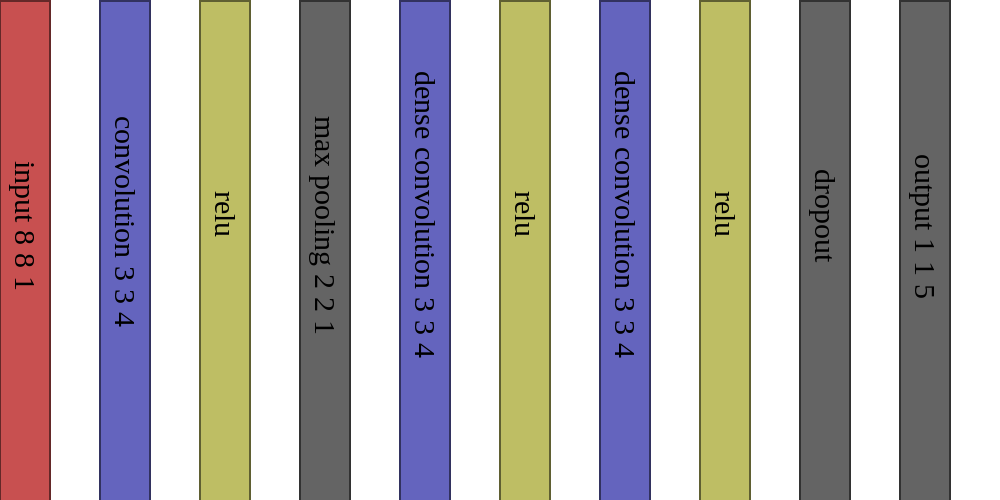
\includegraphics[scale=0.2]{../../diagrams/line_following_net.png}
\end{figure}

\end{frame}




\begin{frame}{\bf Networks results}

{\footnotesize

    \begin{table}[]
    \begin{tabular}{|l|c|c|c|c|}
    \hline
    \textbf{layer}           & \textbf{net 0} & \textbf{net 1} & \textbf{net 2} & \textbf{net 3} \\ \hline
    \textbf{success [\%]}     & 94.04          & 93.92          & 94.96          & 96.32          \\ \hline
    \textbf{FLOPS}           & 7754           & 13354          & 13578          & 25546          \\ \hline
    \textbf{success / FLOPS} & 0.01213        & 0.00703        & 0.00699        & 0.00377        \\ \hline
    \end{tabular}
    \end{table}
}

{\large \bf net 2 confusion matrix}

{\footnotesize

\begin{table}[]
\begin{tabular}{|l|l|l|l|l|l|}
\hline
\textbf{class}         & \textbf{0}     & \textbf{1}   & \textbf{2}   & \textbf{3}   & \textbf{4}   \\ \hline
\textbf{0}             & \textbf{520}   & 8            & 0            & 0            & 0            \\ \hline
\textbf{1}             & 12             & \textbf{453} & 15           & 0            & 0            \\ \hline
\textbf{2}             & 0              & 12           & \textbf{483} & 10           & 0            \\ \hline
\textbf{3}             & 0              & 0            & 15           & \textbf{461} & 53           \\ \hline
\textbf{4}             & 0              & 0            & 0            & 1            & \textbf{457} \\ \hline
                       &                &              &              &              &              \\ \hline
\textbf{class success [\%]} & 97.744         & 95.772       & 94.152       & 97.669       & 89.608       \\ \hline
\textbf{total success [\%]} & \textbf{94.96} &              &              &              &              \\ \hline
\end{tabular}
\end{table}


}
\end{frame}


\begin{frame}{\bf Fitting network into embedded}

convert float weights to int8\_t
\begin{align*}
  scale &= max{(|\vec{w}|_1)} \\
  \vec{w}' &= \vec{w}\frac{127}{scale}
\end{align*}


use double buffer memory trick

\begin{itemize}
  \item unsigned buffer\_size = $\max_{i}$(layers[i].input\_size());
  \item buffer\_a = new int8\_t(buffer\_size);
  \item buffer\_b = new int8\_t(buffer\_size);
\end{itemize}

\begin{figure}
  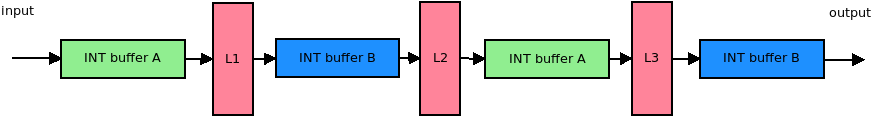
\includegraphics[scale=0.3]{../../diagrams/nn_memory.png}
\end{figure}

\end{frame}




\begin{frame}{\bf Q\&A}

\begin{figure}
  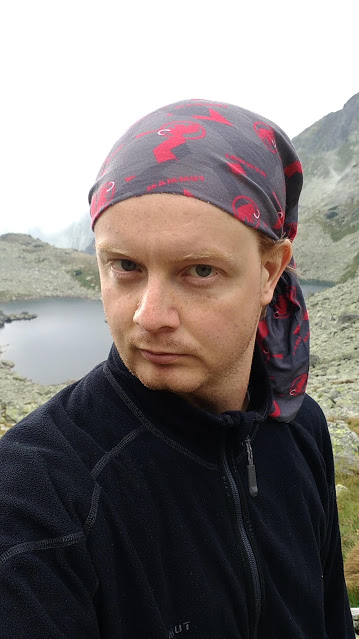
\includegraphics[scale=0.25]{../../pictures/me.jpg}
\end{figure}

\centering {
michal chovanec (michal.nand@gmail.com)
\url{www.youtube.com/channel/UCzVvP2ou8v3afNiVrPAHQGg}
}

\centering {
github
\url{https://github.com/michalnand}
}

\end{frame}


\end{document}
